\documentclass[11pt]{article}

% ------
% LAYOUT
% ------
\textwidth 165mm %
\textheight 230mm %
\oddsidemargin 0mm %
\evensidemargin 0mm %
\topmargin -15mm %
\parindent= 10mm

\usepackage[dvips]{graphicx}
\usepackage{multirow,multicol}
\usepackage[table]{xcolor}

\usepackage{amssymb}
\usepackage{amsfonts}
\usepackage{amsthm}
\usepackage{amsmath}

\usepackage{subfigure}
\usepackage{minted}

\graphicspath{{./pix/}} % put all your figures here.

\begin{document}
\begin{center}
\Large{\textbf{ECE 595: Homework 5}}

Yi Qiao, Class ID 187

(Spring 2019)
\end{center}

\section*{Exercise 1: Adversarial Attacks on Gaussian Classifier}
\subsection*{(a) minimum-norm attacks}
\subsubsection*{(i) minimum $l_2$ and $l_\infty$ attack}
Since we only have 2 classes, the question becomes
\begin{equation}
\begin{split}
&\underset{\pmb{x}}{minimize}\ ||\pmb{x} - \pmb{x}_0||\\
&subject\ to\ \pmb{w}^T\pmb{x} + w_0 = 0
\end{split}
\end{equation}
\noindent\textbf{using $l_2$ norm}\\
the problem is the same as\\
\begin{equation}
\begin{split}
&\underset{\pmb{x}}{minimize}\ \frac{1}{2}||\pmb{x} - \pmb{x}_0||^2_2\\
&subject\ to\ \pmb{w}^T\pmb{x} + w_0 = 0
\end{split}
\end{equation}
The lagrangian is
\begin{equation}
\begin{split}
\mathcal{L}(\pmb{x},\lambda) &= \frac{1}{2}||\pmb{x}-\pmb{x}_0||^2_2 + \lambda(\pmb{w}^T\pmb{x} + w_0)\\
\end{split}
\end{equation}
Taking the derivative
\begin{equation}
\begin{split}
&\nabla_{\pmb{x}}\mathcal{L}(\pmb{x},\lambda) = \pmb{x} - \pmb{x}_0 + \lambda\pmb{w}=0\\
&\frac{\partial}{\partial\lambda}\mathcal{L}(\pmb{x},\lambda)=\pmb{w}^T\pmb{x} + w_0=0
\end{split}
\end{equation}
\begin{equation}
\begin{split}
\lambda\pmb{w}&=\pmb{x}_0 - \pmb{x}\\
\lambda\pmb{w}^T\pmb{w} &= \pmb{w}^T\pmb{x}_0-\pmb{w}^T\pmb{x}\\
\lambda &= \left(\pmb{w}^T\pmb{w}\right)^{-1}(\pmb{w}^T\pmb{x}_0+w_0)
\end{split}
\end{equation}
\begin{equation}
\begin{split}
\pmb{x} &= \pmb{x}_0-\lambda\pmb{w}\\
&=\pmb{x}_0-\frac{\pmb{w}(\pmb{w}^T\pmb{x}_0+w_0)}{||\pmb{w}||_2^2}
\end{split}
\end{equation}
\noindent\textbf{using $l_\infty$ norm}\\
\begin{equation}
\begin{split}
&\underset{\pmb{x}}{minimize}\ ||\pmb{x} - \pmb{x}_0||_{\infty}\\
&subject\ to\ \pmb{w}^T\pmb{x} + w_0 = 0
\end{split}
\end{equation}
Let $\pmb{r} = \pmb{x} - \pmb{x}_0$, $b_0 = -(\pmb{w}^T\pmb{x}_0+w_0)$, the problem becomes:
\begin{equation}
\begin{split}
&\underset{\pmb{x}}{argmin}||\pmb{x}-\pmb{x}_0||_\infty\\
&subject\ to\ \pmb{w}^T\pmb{r}=b_0
\end{split}
\end{equation}
The lagrangian is
\begin{equation}
\begin{split}
\mathcal{L}(\pmb{r},\lambda)=||\pmb{r}||_{\infty}+\lambda(b_0-\pmb{w}^T\pmb{r})
\end{split}
\end{equation}
Taking derivative,
\begin{equation}
\frac{\partial}{\partial\lambda}\mathcal{L}(\pmb{r},\lambda)=b_0-\pmb{w}^T\pmb{r}=0
\end{equation}
By Holder's Inequality:
\begin{equation}
\begin{split}
|b_0|=|\pmb{w}^T\pmb{r}| &\le||\pmb{w}||_1||\pmb{r}||_\infty\\
||\pmb{r}||_\infty&\ge\frac{|b_0|}{||\pmb{w}||_1}
\end{split}
\end{equation}
Consider $\pmb{r}=\eta \cdot sign(\pmb{w})$, for some constant $\eta$ tbd.
We can show that
\begin{equation}
\begin{split}
||\pmb{r}||_\infty = \underset{i}{argmax}\ |\eta\cdot sign(w_i)|=|\eta|
\end{split}
\end{equation}
let $\eta=\frac{b_0}{||\pmb{w}||_1}\cdot sign(\pmb{w})$, then we have,
\begin{equation}
||\pmb{r}||_\infty = |\eta| = \frac{b_0}{||\pmb{w}||_1}
\end{equation}
Lower bound is achieved, thus the solution is,
\begin{equation}
\pmb{r}=\frac{|b_0|}{||\pmb{w}_1||}\cdot sign(\pmb{w})
\end{equation}
\subsubsection*{(ii) DeepFool attack}
\begin{equation}
\begin{split}
&\underset{\pmb{x}}{argmin}\ ||\pmb{x}-\pmb{x}_0||^2_2\\
&subject\ to\ g(\pmb{x})=0
\end{split}
\end{equation}
First order approximation
\begin{equation}
g(\pmb{x})\approx g(\pmb{x}^{(k)})+\nabla_{\pmb{x}}g(\pmb{x}^{(k)})^T(\pmb{x}-\pmb{x}^{(k)})
\end{equation}
Then the problem can be approximate by
\begin{equation}
\begin{split}
&\underset{\pmb{x}}{argmin}\ ||\pmb{x}-\pmb{x}_0||^2_2\\
&subject\ to\ g(\pmb{x}^{(k)})+\nabla_{\pmb{x}}g(\pmb{x}^{(k)})^T(\pmb{x}-\pmb{x}^{(k)})=0
\end{split}
\end{equation}
Let $\pmb{w}^{(k)}=\nabla_{\pmb{x}}g(\pmb{x}^{(k)})$ and $w_0^{(k)}=g(\pmb{x}^{(k)})-\nabla_{\pmb{x}}g(\pmb{x}^{(k)})^T\pmb{x}^{(k)}$\\
Then the problem is equivalent to 
\begin{equation}
\begin{split}
&\underset{\pmb{x}}{argmin}\ ||\pmb{x}-\pmb{x}_0||^2_2\\
&subject\ to\ (\pmb{w}^{(k)})^T\pmb{x}+w_0^{(k)}=0
\end{split}
\end{equation}
This is the same problem as minimum $l_2$ norm attack, Thus the solution will be,
\begin{equation}
\pmb{x}^{(k+1)}=\pmb{x}^{(k)}-\frac{((\pmb{w}^{(k)})^Tx^{(k)} + w_0^{(k)})\pmb{w}^{(k)}}{||\pmb{w}^{(k)}||^2_2}
\end{equation}
substitute $\pmb{w}$ and $w_0$ back, we get
\begin{equation}
\pmb{x}^{(k+1)}=\pmb{x}^{(k)}-\left(\frac{g(\pmb{x}^{(k)})}{||\nabla_{\pmb{x}}g(\pmb{x}^{(k)})||^2}\right)\nabla_{\pmb{x}}g(\pmb{x}^{(k)})
\end{equation}
\subsubsection*{(iii) An example DeepFool never converge}
\begin{figure}[h]
	\centering
	\includegraphics[width=0.5\linewidth]{exercise1_a2}
	\caption{1D example classifier}
\end{figure}
Above is a example discriminate function $g(x)$. there are two classes, separated by the vertical line at $g(x)=0$. If $x_0$ at the position shown above, the Deep Fool attack will result in $x_{attack}$ in the end, and thus never converge to $g(x)=0$.
\subsection*{(b) maximum-allowable attack}
\subsubsection*{(i) $l_\infty$ attack in the linear case}
The problem is,
\begin{equation}
\begin{split}
&\underset{\pmb{x}}{argmin}\ \pmb{w}^T\pmb{x}+w_0\\
&subject\ to\ ||\pmb{x}-\pmb{x}_0||_\infty<\eta
\end{split}
\end{equation}
let $\pmb{x}=\pmb{x}_0+\pmb{r}$, $b_0=(\pmb{w}^T\pmb{x}_0+w_0)$, the problem becomes,
\begin{equation}
\begin{split}
&\underset{\pmb{r}}{argmin}\ \pmb{w}^T\pmb{r}+b_0\\
&subject\ to\ ||\pmb{r}||_\infty<\eta
\end{split}
\end{equation}
by Holder's inequality,
\begin{equation}
\begin{split}
\pmb{w}^T\pmb{r} \ge -||\pmb{r}||_\infty||\pmb{w}||_1\ge-\eta||\pmb{w}||_1
\end{split}
\end{equation}
as shown in the lecture note, the solution 
\begin{equation}
\pmb{r} = -\eta\cdot sign(\pmb{w})
\end{equation}
\subsubsection*{(ii) FGSM attack}
\begin{equation}
\begin{split}
&\underset{\pmb{x}}{argmax}\ J(\pmb{x},\pmb{w})\\
&subject\ to\ ||\pmb{x}-\pmb{x}_0||_\infty\le\eta
\end{split}
\end{equation}
Approximately, $J(\pmb{x},\pmb{w}) = J(\pmb{x}_0+\pmb{r},\pmb{w})\approx J(\pmb{x}_0, \pmb{w})+\nabla_{\pmb{x}}J(\pmb{x}_0,\pmb{w})^T\pmb{r}$\\
Then, the problem becomes
\begin{equation}
\begin{split}
&\underset{\pmb{x}}{argmin}\ -J(\pmb{x}_0, \pmb{w})-\nabla_{\pmb{x}}J(\pmb{x}_0,\pmb{w})^T\pmb{r}\\
&subject\ to\ ||\pmb{r}||_\infty\le\eta
\end{split}in
\end{equation}
of which the solution is given by
\begin{equation}
\begin{split}
\pmb{x} = \pmb{x}_0+\eta\cdot(\nabla_{\pmb{x}}J(\pmb{x}_0,\pmb{w}))
\end{split}
\end{equation}
In the problem setup, we get $J(\pmb{x})= -g(\pmb{x})$, thus the solution is 
\begin{equation}
\begin{split}
\pmb{x} &= \pmb{x}_0-\eta\cdot(\nabla_{\pmb{x}}g(\pmb{x}_0))\\
&= \pmb{x}_0-\eta\cdot((\pmb{W}_j-\pmb{W}_t)\pmb{x}_0+(\pmb{w}_j-\pmb{w}_t))\\
&= (\eta(\pmb{W}_t-\pmb{W}_j)+1)\pmb{x}_0+\eta(\pmb{w}_t-\pmb{w}_j)
\end{split}
\end{equation}
\subsubsection*{(iii) I-FGSM attack}

\begin{equation}
\begin{split}
J(\pmb{x},\pmb{w})&=J(\pmb{x}_0+\pmb{r},\pmb{w})\\
&\approx J(\pmb{x}_0,\pmb{w})+\nabla_{\pmb{x}}J(\pmb{x}_0,\pmb{w})^T\pmb{r}\\
&= J(\pmb{x}_0,\pmb{w})+\nabla_{\pmb{x}}J(\pmb{x}_0,\pmb{w})^T(\pmb{x}-\pmb{x}_0)\\
&= J(\pmb{x}_0,\pmb{w})+\nabla_{\pmb{x}}J(\pmb{x}_0,\pmb{w})^T\pmb{x}-\nabla_{\pmb{x}}J(\pmb{x}_0,\pmb{w})^T\pmb{x}_0\\
\end{split}
\end{equation}

\begin{equation}
\begin{split}
\pmb{x}^{(k+1)}&=\underset{0\le \pmb{x}\le 1}{argmax}\ J(\pmb{x}^{(k)},\pmb{w})\ subject\ to\ ||\pmb{x}-\pmb{x}_0||\le\eta\\
&=\underset{0\le \pmb{x}\le 1}{argmax}\ \nabla_{\pmb{x}}J(\pmb{x}^{(k)},\pmb{w})^T\pmb{x}\ subject\ to\ ||\pmb{x}-\pmb{x}_0||\le\eta\\
&=\mathcal{P}\left\{\pmb{x}^{(k)}+\eta\cdot sign\left(\nabla_{\pmb{x}}J(\pmb{x}^{(k)},\pmb{w})\right)\right\}
\end{split}
\end{equation}

\subsection*{(c) Regularization based attack}
\subsubsection*{(i) linear case}
\begin{equation}
\underset{\pmb{x}}{argmin}\ \frac{1}{2}||\pmb{x}-\pmb{x}_0||^2_2+\lambda(\pmb{w}^T\pmb{x}+w_0)
\end{equation}
Taking derivative
\begin{equation}
\begin{split}
&\nabla_{\pmb{x}}\ \frac{1}{2}||\pmb{x}-\pmb{x}_0||^2_2+\lambda(\pmb{w}^T\pmb{x}+w_0)\\
&=\pmb{x}-\pmb{x}_0+\lambda\pmb{w} = 0
\end{split}
\end{equation}
Solve for $\pmb{x}$,
\begin{equation}
\pmb{x} = \pmb{x}_0-\lambda\pmb{w}
\end{equation}
\subsubsection*{(ii)}
\begin{equation}
\begin{split}
&\underset{\pmb{x}}{argmin}\ \varphi(\pmb{x}), where\\
&\varphi(\pmb{x})=||\pmb{x}-\pmb{x}_0||^2_2+\lambda\zeta(g_j(\pmb{x})-g_t(\pmb{x})),\\
&\zeta(y)=max(y,0),\ and\ j\ne t
\end{split}
\end{equation}
Taking the derivative,
\begin{equation}
\nabla \varphi(\pmb{x}) = 2(\pmb{x}-\pmb{x}_0)+\lambda\mathbb{I}\{g_j(\pmb{x})-g_t(\pmb{x}) > 0\}\cdot(\nabla_{\pmb{x}}g_j(\pmb{x})-\nabla_{\pmb{x}}g_t(\pmb{x}))\\
\end{equation}
Using my favorite gradient descent, we can tell,
\begin{equation}
\pmb{x}^{(k+1)}=\pmb{x}^{(k)}-\alpha\nabla_{\pmb{x}}\varphi(\pmb{x}^{(k)})
\end{equation}
substituting in $g(\pmb{x})=\frac{1}{2}\pmb{x}^T(\pmb{W}_j-\pmb{W}_t)\pmb{x}+(\pmb{w}_j-\pmb{w}_t)^T\pmb{x}+(w_{j,0}-w_{t,0})$,
we get 
\begin{equation}
\begin{split}
\nabla_{\pmb{x}}g(\pmb{x})&=(\pmb{W}_j-\pmb{W}_t)\pmb{x}+(\pmb{w}_j-\pmb{w}_t)\\
\pmb{x}^{(k+1)}&=\pmb{x}^{(k)}-2\alpha(\pmb{x}^{(k)}-\pmb{x}_0)-\alpha\lambda\mathbb{I}\{g(\pmb{x}) > 0\}\cdot(\nabla_{\pmb{x}}g(\pmb{x}))\\
&=\pmb{x}^{(k)}-2\alpha(\pmb{x}^{(k)}-\pmb{x}_0)-\alpha\lambda\mathbb{I}\{g(\pmb{x}) > 0\}\cdot((\pmb{W}_j-\pmb{W}_t)\pmb{x}+(\pmb{w}_j-\pmb{w}_t))
\end{split}
\end{equation}
\section*{Exercise 2: CW-Attack on Gaussian Classifier - Non-overlapping Patches} 
\subsection*{(a)\&(b) Implementation}
refer to code in the back
\subsection*{(c) Results}
\subsubsection*{(i) \& (ii) The final perturbed images \& their perturbation respectively}
\begin{figure}[h]
	\centering
	\subfigure[$\lambda=1$]{
		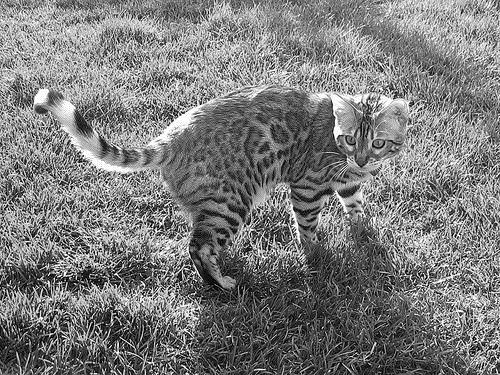
\includegraphics[width=0.3\linewidth]{CW_Nonoverlap_1}
	}
	\subfigure[$\lambda=5$]{
		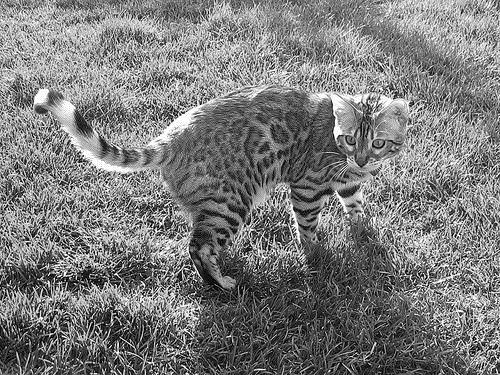
\includegraphics[width=0.3\linewidth]{CW_Nonoverlap_5}
	}
	\subfigure[$\lambda=10$]{
		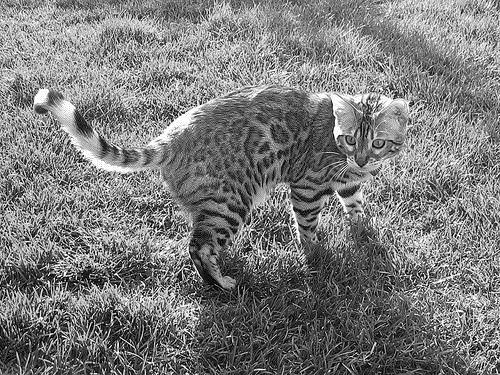
\includegraphics[width=0.3\linewidth]{CW_Nonoverlap_10}
	}
	\subfigure[$\lambda=1$]{
		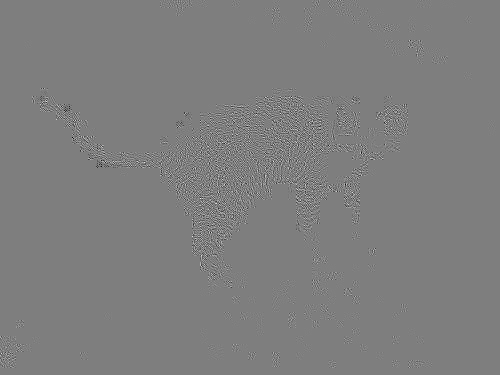
\includegraphics[width=0.3\linewidth]{CW_Nonoverlap_1_perturbation}
	}
	\subfigure[$\lambda=5$]{
		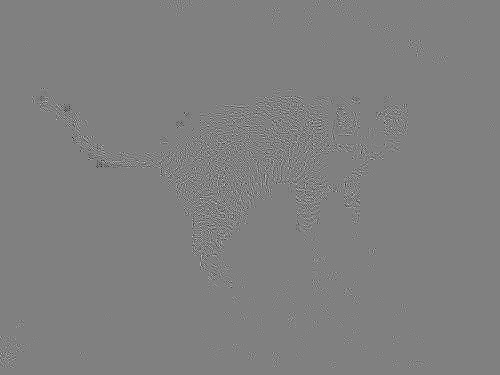
\includegraphics[width=0.3\linewidth]{CW_Nonoverlap_5_perturbation}
	}
	\subfigure[$\lambda=10$]{
		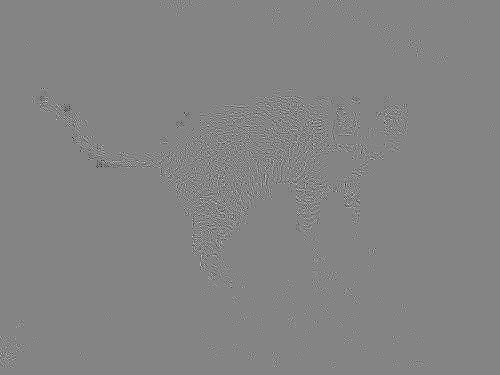
\includegraphics[width=0.3\linewidth]{CW_Nonoverlap_10_perturbation}
	}
	\caption{perturbed images and their perturbations with $\lambda = 1, 5, 10$}
\end{figure}
\subsubsection*{(iii) Frobenius norm of the perturbation}
\begin{table}[h]
	\centering
	\begin{tabular}{c|c|c|c}
		$\lambda$ & 1 & 5 & 10 \\
		\hline
		Frobenius norm & 8.253352243144604 & 8.928742803780679 & 9.697938770929634\\
	\end{tabular}
	\caption{Frobenius norm vs. $\lambda$ for CW-Attack on Gaussian classifier with non-overlapping patches}
\end{table}
\pagebreak
\subsubsection*{(iv) The classifier’s output}
\begin{figure}[h]
	\centering
	\subfigure[$\lambda=1$]{
		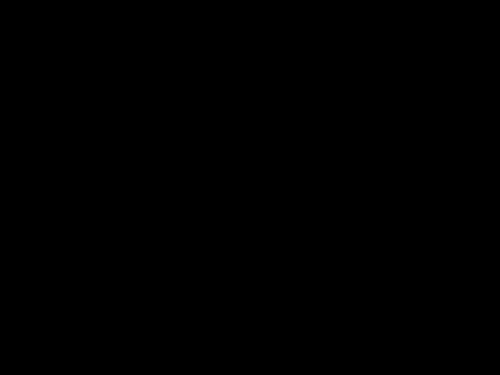
\includegraphics[width=0.3\linewidth]{CW_Nonoverlap_1_classified_pertub}
	}
	\subfigure[$\lambda=5$]{
		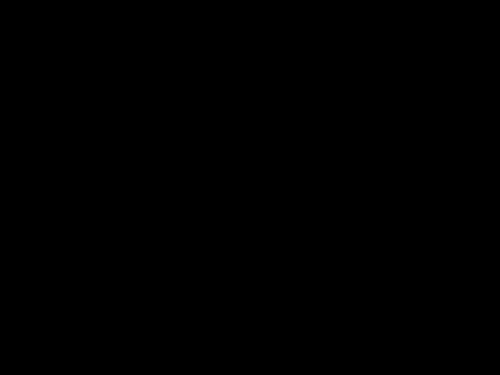
\includegraphics[width=0.3\linewidth]{CW_Nonoverlap_5_classified_pertub}
	}
	\subfigure[$\lambda=10$]{
		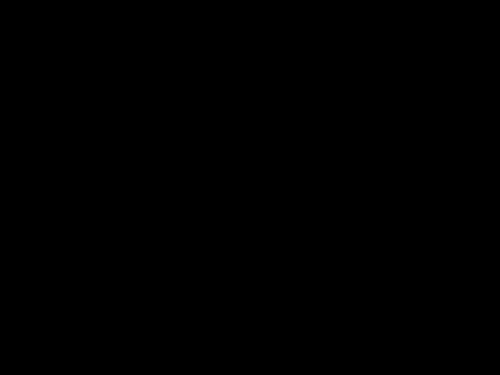
\includegraphics[width=0.3\linewidth]{CW_Nonoverlap_10_classified_pertub}
	}
	\caption{classified perturbed image with $\lambda = 1, 5, 10$}
\end{figure}
For all three cases, all patches are classified as grass after applying perturbation.

\subsubsection*{(v) Plots during gradient descent}
\begin{figure}[h]
	\centering
	\subfigure[after 0 rounds]{
		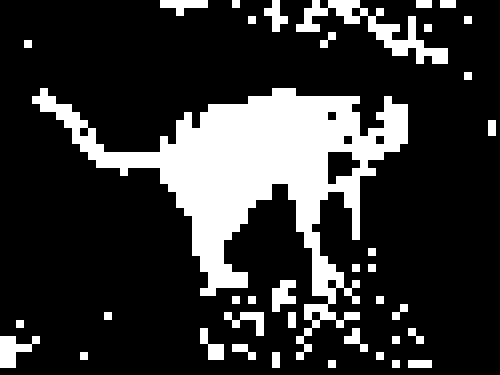
\includegraphics[width=0.3\linewidth]{CW_Nonoverlap_1_r0}
	}
	\subfigure[after 50 rounds]{
		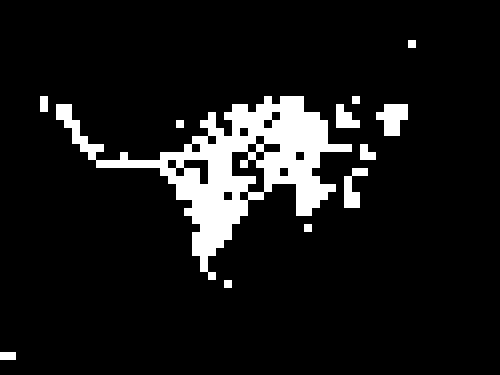
\includegraphics[width=0.3\linewidth]{CW_Nonoverlap_1_r50}
	}
	\subfigure[after 100 rounds]{
		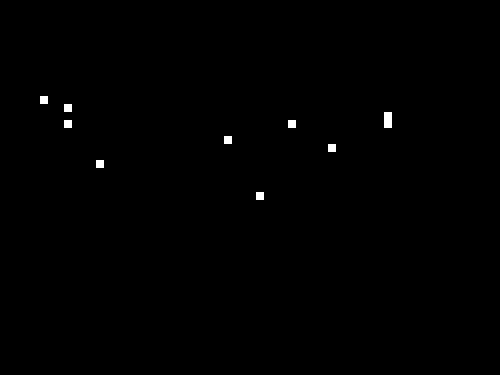
\includegraphics[width=0.3\linewidth]{CW_Nonoverlap_1_r100}
	}
	\caption{classified perturbed image during gradient descent with $\lambda = 1$}
\end{figure}
\begin{figure}[h]
	\centering
	\subfigure[after 0 rounds]{
		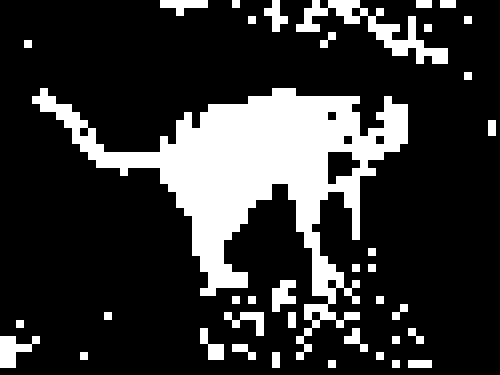
\includegraphics[width=0.3\linewidth]{CW_Nonoverlap_5_r0}
	}
	\subfigure[after 10 rounds]{
		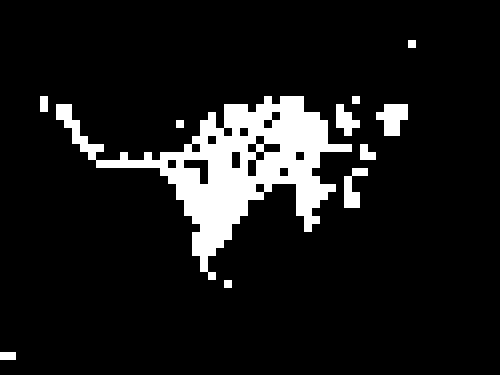
\includegraphics[width=0.3\linewidth]{CW_Nonoverlap_5_r10}
	}
	\subfigure[after 20 rounds]{
		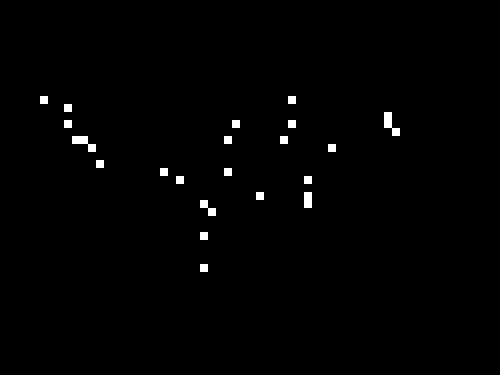
\includegraphics[width=0.3\linewidth]{CW_Nonoverlap_5_r20}
	}
	\caption{classified perturbed image during gradient descent with $\lambda = 5$}
\end{figure}
\pagebreak
\begin{figure}[h]
	\centering
	\subfigure[after 0 rounds]{
		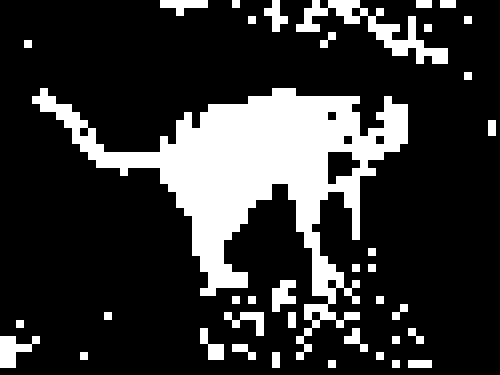
\includegraphics[width=0.21\linewidth]{CW_Nonoverlap_10_r0}
	}
	\subfigure[after 5 rounds]{
		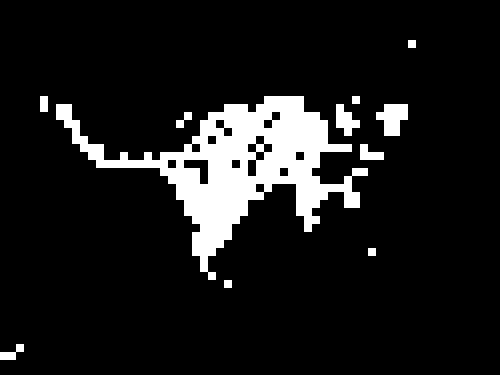
\includegraphics[width=0.21\linewidth]{CW_Nonoverlap_10_r5}
	}
	\subfigure[after 10 rounds]{
		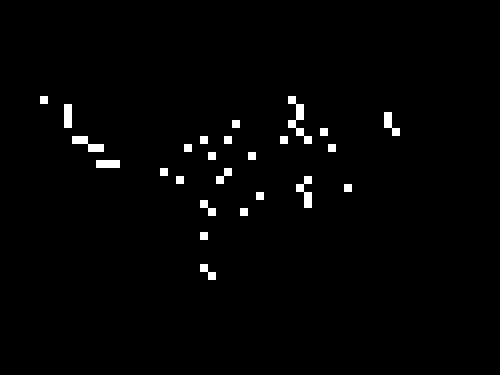
\includegraphics[width=0.21\linewidth]{CW_Nonoverlap_10_r10}
	}
	\subfigure[after 15 rounds]{
		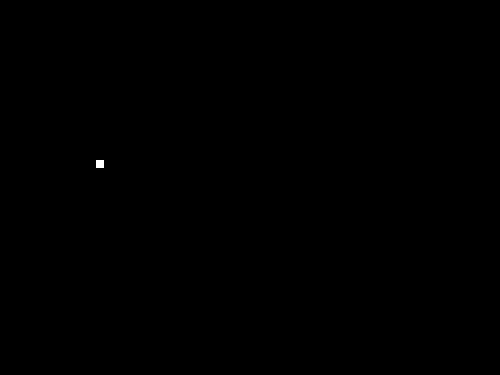
\includegraphics[width=0.21\linewidth]{CW_Nonoverlap_10_r15}
	}
	\caption{classified perturbed image during gradient descent with $\lambda = 10$}
\end{figure}

\subsection*{Comments}
From the above plots, we can obviously see that increase $\lambda$ will speed up the attack. However, as $\lambda$ goes up, the quality of the attack goes down since the Frobenius norm also goes up while achieving the same result.
\pagebreak
\section*{Exercise 3: CW Attack on Gaussian Classifier - Overlapping Patches}
\begin{equation}
\begin{split}
\pmb{X}^*&=\underset{\pmb{X}}{argmin}\sum_{i=1}^{L}\{||\pmb{P}_i(\pmb{X}-\pmb{X}_0)||^2_2+\lambda max(g_j(\pmb{P}_i\pmb{X})-g_t(\pmb{P}_i\pmb{X}),0)\}\\
&=\underset{\pmb{X}}{argmin}||\pmb{X}-\pmb{X}_0||^2_2+\lambda\sum_{i=1}^{L}max(g_j(\pmb{P}_i\pmb{X})-g_t(\pmb{P}_i\pmb{X}),0)
\end{split}
\end{equation}
\subsection*{(a) Theory} the gradient of the above function is,
\begin{equation}
\begin{split}
\nabla_{\pmb{X}}=2(\pmb{X}-\pmb{X}_0)+\lambda\mathbb{I}\{g_j(\pmb{P}_i\pmb{X})-g_t(\pmb{P}_i\pmb{X})>0\}\times(\nabla_{\pmb{X}}(g_j(\pmb{P}_i\pmb{X})-g_t(\pmb{P}_i\pmb{X})))
\end{split}
\end{equation} 
\subsection*{(b) Implementation}
Refer to code in the back.
\subsection*{(c) Results}
\subsubsection*{(i) \& (ii) The final perturbed images \& their perturbation respectively}
\begin{figure}[h]
	\centering
	\subfigure[$\lambda=0.5$]{
		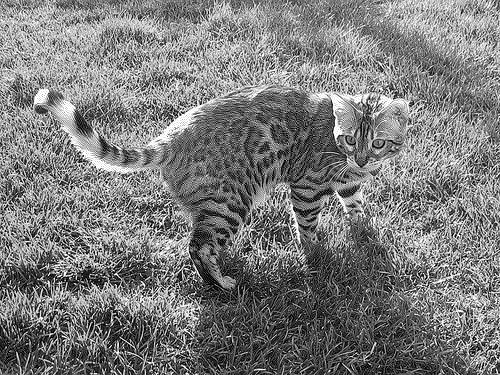
\includegraphics[width=0.3\linewidth]{CW_Overlap_5}
	}
	\subfigure[$\lambda=1.0$]{
		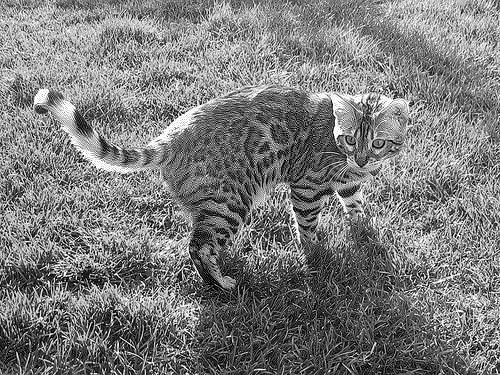
\includegraphics[width=0.3\linewidth]{CW_Overlap_10}
	}
	\subfigure[$\lambda=5.0$]{
		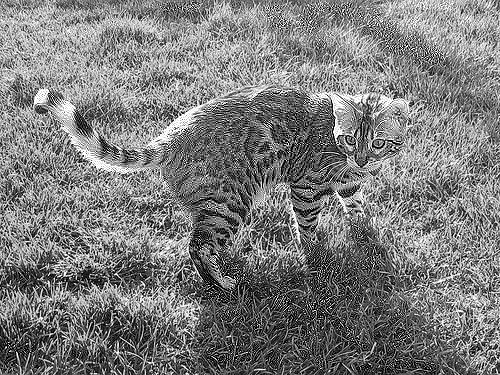
\includegraphics[width=0.3\linewidth]{CW_Overlap_50}
	}
	\subfigure[$\lambda=0.5$]{
		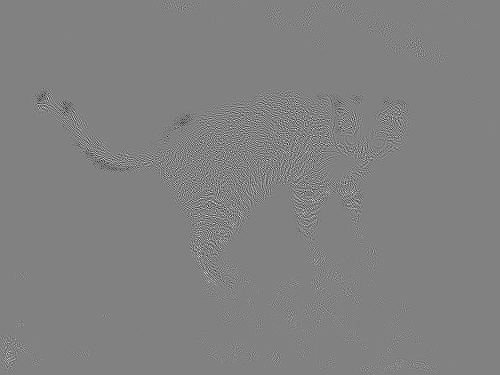
\includegraphics[width=0.3\linewidth]{CW_Overlap_5_perturbation}
	}
	\subfigure[$\lambda=1.0$]{
		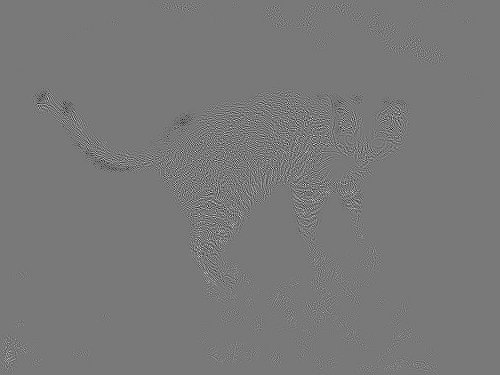
\includegraphics[width=0.3\linewidth]{CW_Overlap_10_perturbation}
	}
	\subfigure[$\lambda=5.0$]{
		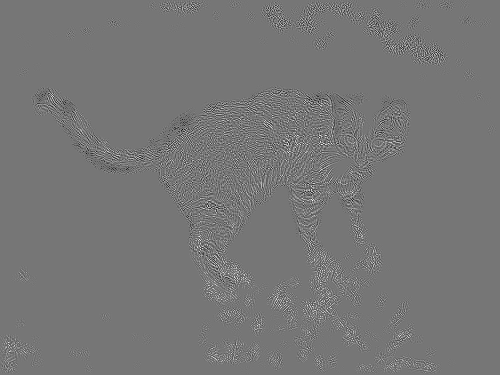
\includegraphics[width=0.3\linewidth]{CW_Overlap_50_perturbation}
	}
	\caption{perturbed images and their perturbations with $\lambda = 0.5, 1.0, 5.0$}
\end{figure}
\pagebreak
\subsubsection*{(iii) Frobenius norm of the perturbation}
\begin{table}[h]
	\centering
	\begin{tabular}{c|c|c|c}
		
		$\lambda$ & \#grass patches & \#cat patches & Frobenius norm\\ 
		\hline\hline
		0.5 & 180561 & 3 & 14.059260687697552 \\  
		1.0 & 180561 & 3 & 16.158563208747122 \\
		5.0 & 180564 & 0 & 33.617113348842395
	\end{tabular}
	\caption{testing results for CW-Attack on Gaussian classifier with overlapping patches}
\end{table}
\subsubsection*{(iv) The classifier’s output}
\begin{figure}[h]
	\centering
	\subfigure[$\lambda=0.5$]{
		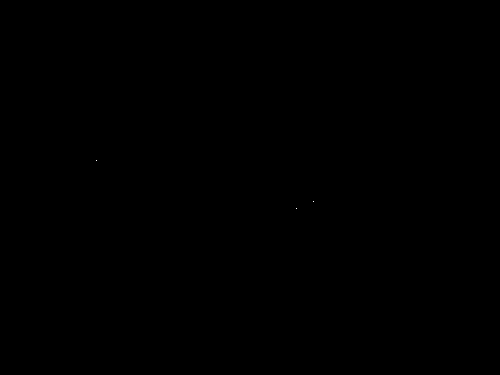
\includegraphics[width=0.3\linewidth]{CW_Overlap_5_classified_perturb}
	}
	\subfigure[$\lambda=1.0$]{
		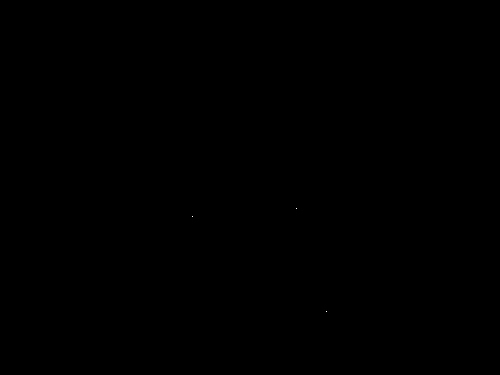
\includegraphics[width=0.3\linewidth]{CW_Overlap_10_classified_perturb}
	}
	\subfigure[$\lambda=5.0$]{
		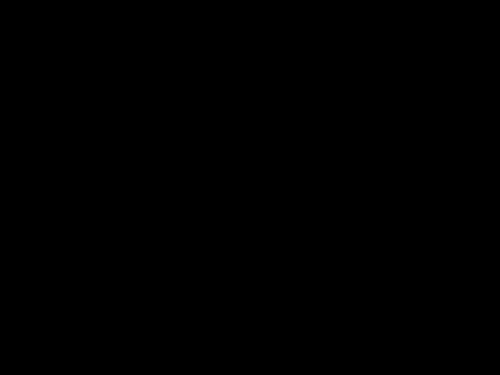
\includegraphics[width=0.3\linewidth]{CW_Overlap_50_classified_perturb}
	}
	\caption{classified perturbed image with $\lambda = 0.5, 1.0, 5.0$}
\end{figure}
The precise result is in the table above, however, from observation, almost all pixels are classified as grass.
\subsubsection*{(v) Plots during gradient descent}
\begin{figure}[h]
	\centering
	\subfigure[after 0 rounds]{
		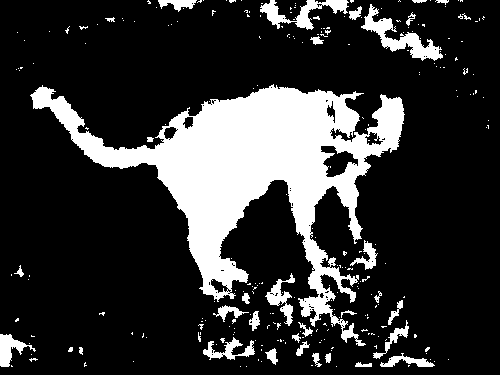
\includegraphics[width=0.21\linewidth]{CW_Overlap_5_r0}
	}
	\subfigure[after 5 rounds]{
		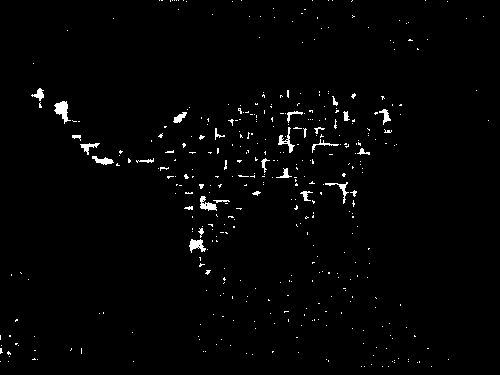
\includegraphics[width=0.21\linewidth]{CW_Overlap_5_r5}
	}
	\subfigure[after 10 rounds]{
		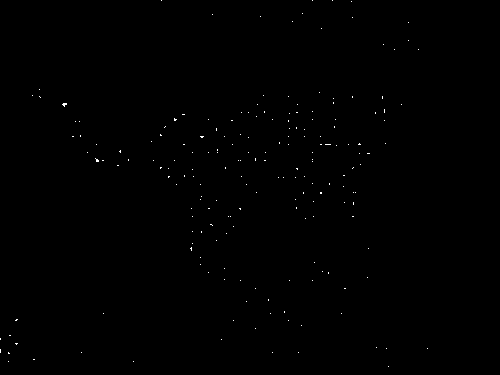
\includegraphics[width=0.21\linewidth]{CW_Overlap_5_r10}
	}
	\subfigure[after 15 rounds]{
		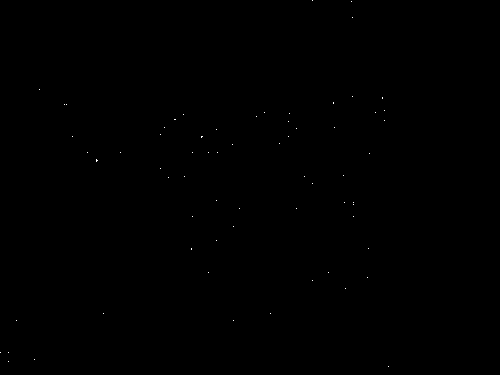
\includegraphics[width=0.21\linewidth]{CW_Overlap_5_r15}
	}
	\subfigure[after 20 rounds]{
		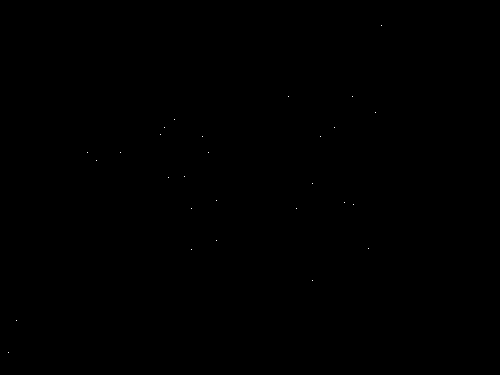
\includegraphics[width=0.21\linewidth]{CW_Overlap_5_r20}
	}
	\subfigure[after 25 rounds]{
		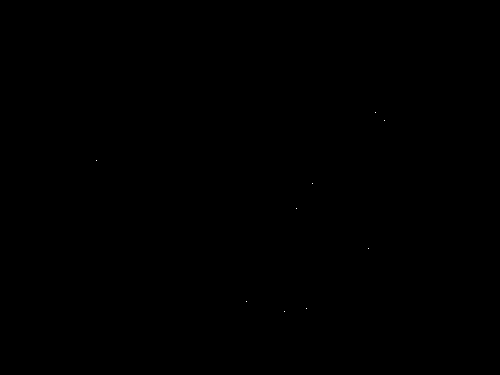
\includegraphics[width=0.21\linewidth]{CW_Overlap_5_r25}
	}
	\subfigure[after 30 rounds]{
		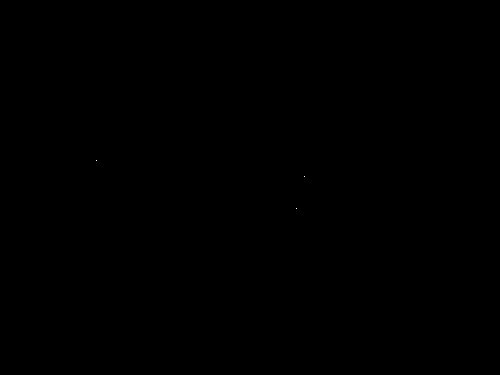
\includegraphics[width=0.21\linewidth]{CW_Overlap_5_r30}
	}
	\caption{classified perturbed image during gradient descent with $\lambda = 0.5$}
\end{figure}
\begin{figure}[h]
	\centering
	\subfigure[after 0 rounds]{
		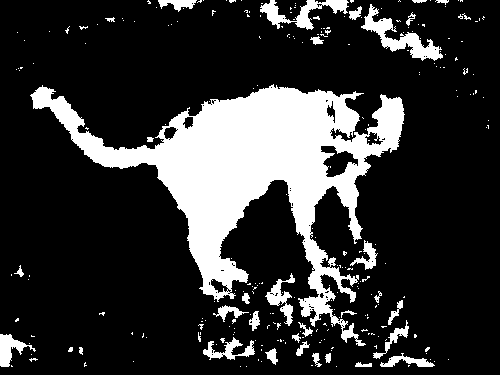
\includegraphics[width=0.21\linewidth]{CW_Overlap_10_r0}
	}
	\subfigure[after 5 rounds]{
		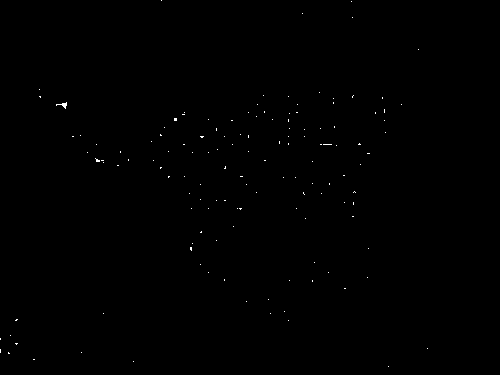
\includegraphics[width=0.21\linewidth]{CW_Overlap_10_r5}
	}
	\subfigure[after 10 rounds]{
		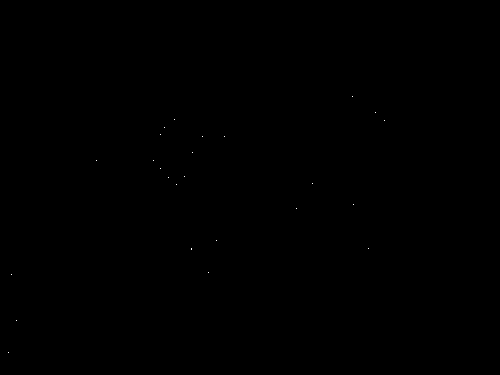
\includegraphics[width=0.21\linewidth]{CW_Overlap_10_r10}
	}
	\subfigure[after 15 rounds]{
		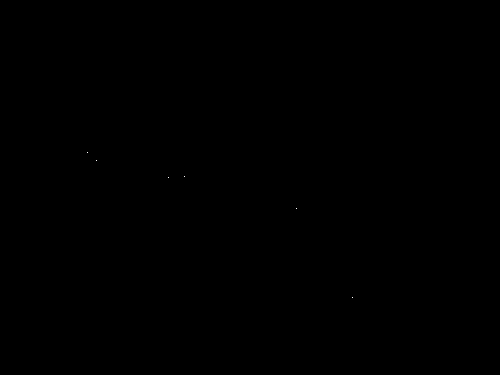
\includegraphics[width=0.21\linewidth]{CW_Overlap_10_r15}
	}
	\caption{classified perturbed image during gradient descent with $\lambda = 1.0$}
\end{figure}
\begin{figure}[h]
	\centering
	\subfigure[after 0 rounds]{
		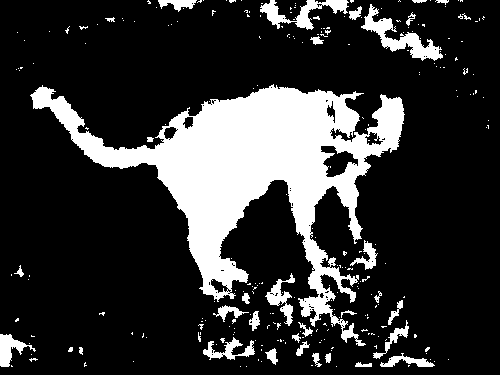
\includegraphics[width=0.21\linewidth]{CW_Overlap_50_r0}
	}
	\subfigure[after 2 rounds]{
		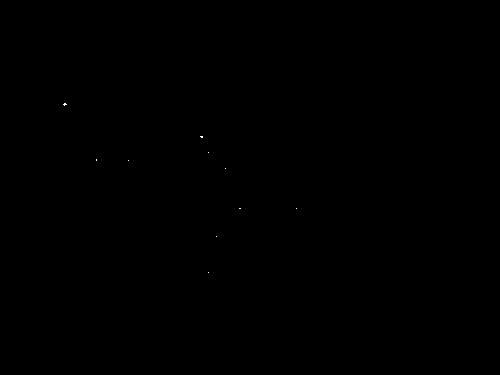
\includegraphics[width=0.21\linewidth]{CW_Overlap_50_r2}
	}
	\subfigure[after 4 rounds]{
		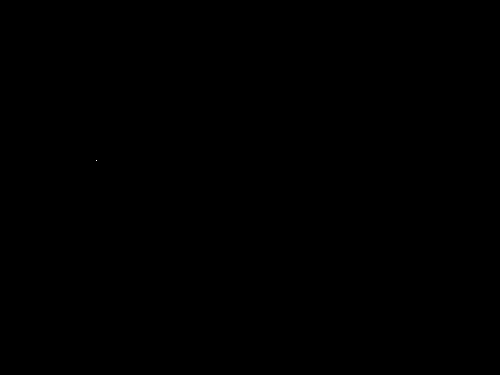
\includegraphics[width=0.21\linewidth]{CW_Overlap_50_r4}
	}
	\caption{classified perturbed image during gradient descent with $\lambda = 5$}
\end{figure}
\pagebreak

\subsection*{Comments}
In general, comparing to the non-overlapping case, the Frobenius norm is significantly larger. However, since the overlapping is a much harder problem, the result is acceptable. As $lambda$ goes up, the strength of the attack is approximately the same, less rounds are needed to attack the classifier while sacrificing some quality of the attack.

\section*{Code}

\subsection*{Exercise 2: CW-Attack on Gaussian Classifier - Non-overlapping Patches}
\inputminted[breaklines]{python}{./py/exercise2.py}
\subsection*{Exercise 3: CW-Attack on Gaussian Classifier - Overlapping Patches}
\inputminted[breaklines]{python}{./py/exercise3.py}
\end{document}